\documentclass{ieeeaccess}
\usepackage{cite}
\usepackage{amsmath,amssymb,amsfonts}
%\usepackage{algorithm}
\usepackage{algorithmic}
\usepackage{units}
\usepackage[ruled, vlined, linesnumbered]{algorithm2e}
\usepackage{graphicx}
\usepackage{textcomp}

\usepackage{enumitem}

%Please add the following packages if necessary:
\usepackage{booktabs, multirow} % for borders and merged ranges
\usepackage{soul}% for underlines
\usepackage[table]{xcolor} % for cell colors
\usepackage{changepage,threeparttable} % for wide tables

\usepackage[commentmarkup=footnote,final]{changes} % Add changes for correction in text. USE THIS FOR FINAL VERSION
%\usepackage[commentmarkup=footnote]{changes} % Add changes for correction in text. USE THIS FOR REVIEW


\newcommand\Fig[1]{\textbf{Fig.}~\ref{#1}}
\newcommand\fig[1]{\textbf{Fig.}~\ref{#1}}
\newcommand\Tab[1]{\textbf{Tab.}~\ref{#1}}
\newcommand\tab[1]{\textbf{Tab.}~\ref{#1}}
\newcommand\Equ[1]{\textbf{Eq.}~(\ref{#1})}
\newcommand\equ[1]{\textbf{Eq.}~(\ref{#1})}
\newcommand\Sect[1]{\textbf{Sec.}~\ref{#1}}
\newcommand\sect[1]{\textbf{Sec.}~\ref{#1}}
\newcommand\Refs[1]{\textbf{Ref.}~\cite{#1}}
\newcommand\refs[1]{\textbf{Ref.}~\cite{#1}}
\newcommand\Algo[1]{\textbf{Algorithm}~\ref{#1}}
\newcommand\algo[1]{\textbf{Algorithm}~\ref{#1}}


\newcommand\todo[1]{\textbf{(TODO: {#1}})\\}

% To highlight "review"
\newcommand\REVIEW[1]{\hl{#1}}
\newcommand\REVIEWR[1]{\colorbox{pink}{#1}}
%To remove highlight
%\newcommand\REVIEW[1]{{#1}}
%\newcommand\REVIEWR[1]{{#1}}

\begin{document}
\history{Date of publication xxxx 00, 0000, date of current version xxxx 00, 0000.}
\doi{10.1109/ACCESS.2017.DOI}


\title {CNN Sensor Analytics with Hybrid-Float6 on Low-Power Resource-Constrained Embedded FPGAs.}


\tfootnote{This work is funded by the Consejo Nacional de Ciencia y Tecnologia - CONACYT}

\markboth
{Author \headeretal: Preparation of Papers for IEEE TRANSACTIONS and JOURNALS}
{Author \headeretal: Preparation of Papers for IEEE TRANSACTIONS and JOURNALS}

\corresp{Corresponding author: Yarib Nevarez (e-mail: nevarez@item.uni-bremen.de).}

\begin{abstract}
The use of artificial intelligence (AI) in sensor analytics is entering a new era based on the use of ubiquitous embedded connected devices. This transformation requires the adoption of design techniques that reconcile accurate results with sustainable system architectures. As such, improving the efficiency of AI hardware engines as well as machine learning (ML) compatibility must be considered. In this paper, we present the Hybrid-Float6 (HF6) quantization and its dedicated hardware design. We propose an optimized multiply-accumulate (MAC) hardware by reducing the mantissa multiplication to a multiplexor-adder operation. We exploit the intrinsic error tolerance of neural networks to further reduce the hardware design with approximation. To preserve model accuracy, we present a quantization-aware training (QAT) method, which in some cases improves accuracy. We demonstrate this concept in 2D convolution layers. We present a lightweight tensor processor (TP) implementing a pipelined vector dot-product. For ML compatibility/portability, the 6-bit FP is wrapped in the standard FP format, which is automatically extracted by the proposed hardware. The hardware/software architecture is compatible with TensorFlow (TF) Lite. We evaluate the applicability of our approach with a CNN-regression model for anomaly localization in a structural health monitoring (SHM) application. The embedded hardware/software framework is demonstrated on XC7Z007S as the smallest Zynq-7000 SoC. The proposed implementation achieves a peak power efficiency and acceleration of $5.7$ GFLOPS/s/W and $48.3\times$, respectively.
\end{abstract}

\begin{keywords}
Convolutional neural networks, structural health monitoring, hardware accelerator, TensorFlow Lite, embedded systems, FPGA, custom floating-point
\end{keywords}

\titlepgskip=-15pt

\maketitle

\section{Introduction}
\label{sec:introduction}
%%% General intro
\IEEEPARstart{T}{here} is a growing demand for ubiquitous AI sensor analytics. Industry 4.0 and smart city infrastructure leverage AI solutions to increase productivity and adaptability\cite{lom2016industry}. These solutions are powered by advances in ML, compute engines, and big data. Hence, improvements of these should be considered for research, as they are the machinery of the future.

Convolutional neural networks (CNNs) represent the essential building blocks in 2D pattern analytics. Sensor-based applications such as mechanical fault diagnosis\cite{li2019sensor,dong2018rolling}, structural health monitoring\cite{nagayama2007structural}, human activity recognition (HAR) \cite{wang2019deep}, hazardous gas detection\cite{kim2017hazardous} have been powered by CNN models in industry and academia. CNN-based models, as one of the main types of artificial neural networks (ANNs), have been widely used in sensor analytics with automatic learning from sensor data \cite{ince2016real, janssens2016convolutional, abdeljaber2017real, guo2016hierarchical}. In this context, CNN models are applied for automatic feature learning, usually, from 1D time series as well as for 2D time-frequency spectrograms. CNN models provide advantages such as local dependency, scale invariance, and noise resilience in analytics\cite{du2014leveraging}. However, these models are computationally intensive and power-hungry. This is particularly challenging for low-power embedded applications in the field of Internet-of-Things (IoT).

For ML inference, dedicated hardware architectures are typically used to enhance compute performance and power efficiency. In terms of computational throughput, graphics processing units (GPUs) offer the highest performance; in terms of power efficiency, ASIC and FPGA solutions are more energy efficient \cite{nurvitadhi2017can}. As a result, numerous commercial ASIC and FPGA accelerators have been proposed, targeting both high performance computing (HPC) for data-centers and embedded systems applications.

However, most FPGA accelerators have been implemented to target mid- to high-range FPGAs for computationally intensive CNN models such as AlexNet, VGG-16, and ResNet-18. The main drawbacks of these implementations are power supply demands, physical dimensions, heat sink requirements, air cooling, and high price. In some cases, these implementations are not feasible for ubiquitous low-power/resource-constrained applications.

To reduce the computational cost for CNN inference there are two types of research \cite{wu2021low}: the first one is deep compression including weight pruning, weight quantization, and compression storage \cite{han2015deep,han2015learning}; the second type of research corresponds to a more efficient data representation, also known as custom quantization for dedicated hardware implementation. In this group, hardware implementations with customized 8-bit floating-point computation have been proposed \cite{mei2017200mhz, wu2021low, lian2019high}. However, these implementations are inadequate for embedded applications, since the target devices are high-end FPGA and PCIe architectures.

More aggressive quantization such as binary \cite{courbariaux2015binaryconnect}, ternary \cite{lin2015neural}, and mixed precision (2-bit activations and ternary weights) \cite{colangelo2018exploration} may suffer from great accuracy loss even with time-consuming retraining. This is inadequate for accurate and reliable data analytics methods in low-power embedded applications.

In this paper, we present the Hybrid-Float6 quantization concept and its dedicated hardware design. In this concept, feature maps are represented by standard 32-bit FP and trainable parameters by 6-bit FP. To preserve model accuracy, we present a quantization-aware training method, which in some cases improves model performance. For ML compatibility/portability, the 6-bit FP is wrapped into the standard FP representation. The dedicated hardware design extracts the 6-bit format automatically and performs the computation. We propose a parameterized tensor processor implementing a pipelined vector dot-product with HF6. The 6-bit FP representation uses 4-bit exponent and 1-bit mantissa. This enables low-power multiply-accumulate (MAC) implementations by reducing the FP mantissa multiplication to a flag operation. This approach reduces energy consumption and resource utilization facilitating on-chip stationary weights on limited footprint devices. The embedded hardware/software architecture is integrated with TensorFlow Lite using delegate interface to accelerate \emph{Conv2D} tensor operations. We evaluate the applicability of our approach with a CNN-regression model and hardware design exploration for sensor analytics of SHM for anomaly localization. The embedded hardware/software framework is demonstrated on XC7Z007S as the smallest and most inexpensive Zynq SoC device, see \Fig{fig:workflow}. To the best of our knowledge, this is the first research addressing 6-bit floating-point quantization on CNN models and its dedicated hardware design.

\begin{figure}[t!]
	\centering
	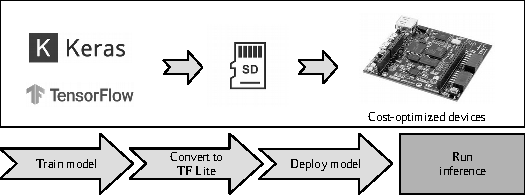
\includegraphics[width=0.5\textwidth]{../figures/workflow.pdf}
	\caption{The workflow of our approach on embedded FPGAs.}
	\label{fig:workflow}
\end{figure}

Our main contributions are as follows:
\begin{enumerate}
	\item
	
	We present the Hybrid-Float6 quantization concept and its dedicated hardware design. To preserve model accuracy, we present a quantization-aware training method, which in some cases improves accuracy.
	
	\item We develop a custom hardware/software co-design framework for sensor analytics applications on low-power embedded FPGAs. This architecture integrates TensorFlow Lite.
	\item We present a customizable tensor processor as a dedicated hardware for HF6. This design computes \emph{Conv2D} tensor operations employing a pipelined vector dot-product with parametrized on-chip memory utilization. The compute engine can be implemented with standard floating-point (with FP Xilinx LogiCORE IPs) and HF6 (with custom logic).
	\item We demonstrate the potential of our approach by addressing a hardware design exploration. We evaluate inference accuracy, compute performance, hardware resource utilization, and energy consumption.
\end{enumerate}

The rest of the paper is organized as follows. Section~\ref{sec:related_work} covers the related work; Section~\ref{sec:background} introduces the background to \emph{Conv2D} and \emph{DepthwiseConv2D} tensor operations; Section~\ref{sec:system_design} describes the system design of the hardware/software architecture and the quantized aware training method; Section~\ref{sec:experimental_results} presents the experimental results thorough a design exploration flow; Section~\ref{sec:conclusions} concludes the paper.

This work is available to the community as an open-source project at https://github.com/YaribNevarez/tensorflow-lite-fpga-delegate.git.
\section{Related work}
\label{sec:related_work}
In the literature we find plenty of hardware architectures for CNN accelerators implemented in FPGA. Most of the research implements fixed-point quantization, and very limited research focuses on FP. Moreover, to the best of our knowledge, there is no research work exploring FP inference for low-power embedded applications.


\subsection{Hybrid Custom Floating-Point}
In \cite{lai2017deep}, Liangzhen Lai et al. proposed a mixed data representation with floating-point for weights and fixed-point for activations. \cite{lai2017deep} demonstrated on SqueezeNet, AlexNet, GoogLeNet, and VGG-16 that reduced FP quantization (4-bit exponent and 3-bit mantissa) results in constant negligible accuracy degradation. In \cite{settle2018quantizing}, Sean O. Settle et al. presented an 8-bit FP quantization scheme, which needs an extra inference batch to compensate for quantization error. However, \cite{lai2017deep} and \cite{settle2018quantizing} did not present a hardware architecture. In \cite{lian2019high}, Xiaocong Lian et al. proposed an accelerator with optimized block floating-point (BFP), in this design the activations and weights are represented by 16-bit and 8-bit FP formats, respectively. This design is demonstrated on Xilinx VC709 evaluation board. This implementation achieves throughput and power efficiency of 760.83 GOP/s and 82.88 GOP/s/W, respectively.

\subsection{Low-Precision Floating-Point}
In \cite{mei2017200mhz}, Chunsheng Mei et al. presented a hardware accelerator for VGG16 model using half-precision FP (16-bit). This design is demonstrated on Xilinx Virtex-7 (XC7VX690T) with PCIe interface. This implementation achieves throughput and power efficiency of 202.8 GFLOP/s and 18.72 GFLOP/s/W, respectively. In \cite{wu2021low}, Chen Wu et al. proposed a low-precision (8-bit) floating-point (LPFP) quantization method for FPGA-based acceleration. This design is demonstrated on Xilinx Kintex 7 and Ultrascale/Ultrascale+. This implementation achieves throughput and power efficiency of 1086.8 GOP/s and 115.4 GOP/s/W, respectively.

\subsection{Low-Power}
Two research papers have been reported hardware accelerators targeting XC7Z007S. This is the smallest and most inexpensive device from Zynq-7000 SoC family. In \cite{meloni2019cnn}, Paolo Meloni et al. presented a CNN inference accelerator for compact and cost-optimized devices. This implementation uses fixed-point for processing light-weight CNN architectures with a power efficiency between 2.49 to 2.98 GOPS/s/W. In \cite{gao2020edgedrnn}, Chang Gao et al. presented EdgeDRNN, a recurrent neural network (RNN) accelerator for edge inference. This implementation adopts the spiking neural network (SNN) inspired delta network algorithm to exploit temporal sparsity in RNNs.
\section{Background}
\label{sec:background}

\subsection{Conv2D tensor operation}
A convolutional layer aims to learn feature representations from an input layer. The convolution layer is made of convolution kernels that are used to compute feature maps. Each unit of a feature map is connected to a region of neighboring units of the input maps (the previous layer). Such a neighborhood of the previous layer is known as the receptive field of the unit. A new feature map can be obtained by first convolving the input maps with a learned kernel and then applying a nonlinear elementwise activation function to the convolved results. All spatial locations in the input maps share a kernel to generate a feature map. All feature maps are obtained by convolving several different kernels\cite{gu2018recent}.


The 2D convolution process is performed by the \emph{Conv2D} tensor operation, described in \Equ{eq:conv2D}, where $h$ is the input feature maps, $W$ is the convolution kernels (known as filters), and $b$ is the bias for the output feature maps\cite{goodfellow2016deep}. We denote \emph{Conv} as \emph{Conv2D} operator.
\begin{eqnarray} \label{eq:conv2D}
Conv\left(W,h\right)_{i,j,o}=\sum_{k,l,m}^{K,L,M} h_{(i+k,j+l,m)} W_{(o,k,l,m)}+b_{o}
\end{eqnarray}

\subsection{Floating-point Number Representation}
The representation of every numerical value, in any number system, is made of an integer and a fractional part. The border that delimits them is called the radix point. The fixed-point format for representing numeric values derives its name from the fact that in this format, the base point is fixed at a certain position. For integer numbers, this position is at the right of the least significant digit.

In scientific computation, it is often necessary to represent very large and very small values. This is difficult to achieve using the fixed point format because the bit size/width required to maintain both the desired precision and the desired range are very large. In such situations, floating-point formats are used to represent real numbers. Each floating-point number can be divided into three fields: sign $S$, exponent $E$, and mantissa $M$. Using the binary number system, it is possible to represent any floating-point number as:

\begin{eqnarray} \label{eq:float}
(-1)^{S} \times 1.M \times 2^{E-B}
\end{eqnarray}

In this representation the exponent is biased, this means that the stored value is offset from 0 by a given value depending on the bit size of the exponent field in the particular format. This exponent bias is defined by \Equ{eq:float_bias}, where $E_{size}$ is the exponent bit size.

\begin{eqnarray} \label{eq:float_bias}
B=2^{E_{size}-1}-1
\end{eqnarray}

There is a natural trade-off between reduced bit size requiring fewer hardware resources and larger bit size providing higher precision. Within a given total bit size, it is possible to assign various combinations of bit widths to the exponent and mantissa fields, with wider exponents resulting in a higher range and wider mantissa resulting in better precision.

The most widely used format for floating-point arithmetic is the IEEE 754 standard \cite{zuras2008ieee}. The IEEE single-precision format (32-bit) is expressed in \Equ{eq:float} with $B$ = 127, 8 bits for the exponent and 23 bits for the mantissa, see \Fig{fig:floating}(a). The numbers are normalized, the leading one is an implicit bit, and only the fractional part is explicitly stored in the mantissa field.

\begin{figure}[h!]
	\centering
	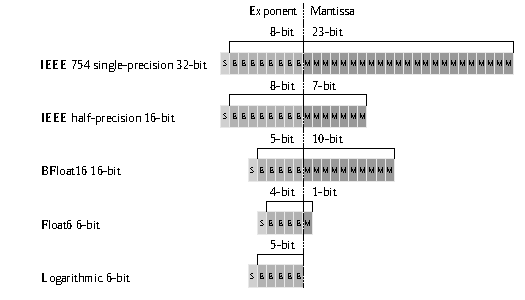
\includegraphics[width=1\columnwidth]{../figures/power_breakdown/floating_point.pdf}
	\caption{Floating-point number representation.}
	\label{fig:floating}
\end{figure}

Reduced bit size than those specified in the IEEE 754 standard are often sufficient to provide the desired precision. Reduced bit size designs require fewer hardware resources enabling low-power implementations. In custom hardware designs, it is possible to customize the exact floating-point format implemented. In later sections, we use the term E$a$M$b$ to denote floating-point representations, where $a$ and $b$ are the exponent and mantissa bit size, respectively. For example, E4M1 means 4-bit exponent and 1-bit mantissa, see \Fig{fig:floating}(d).
\section{System Design}
\label{sec:system_design}
The system design is a hardware/software co-design framework for low-power AI deployment. This architecture allows design exploration of dedicated hardware integrated with TensorFlow Lite on low-cost embedded FPGAs.

\subsection{Base embedded system architecture}
The base embedded system architecture implements a cooperative hardware-software platform. \Fig{fig:system_architecture} illustrates the top-level hardware architecture. The TPs execute low-level tensor operations delegated from the embedded CPU. The TPs employ AXI-Lite interface for configuration and AXI-Stream interfaces via Direct Memory Access (DMA) for data movement from DDR memory. Each TP asserts an interrupt flag once the job/transaction is complete. Interrupt events are handled by the embedded CPU to collect results and start a new transaction. The hardware architecture can configure its resource utilization and energy consumption by customizing the TPs prior to the hardware synthesis.
\begin{figure}[t!]
	\centering
	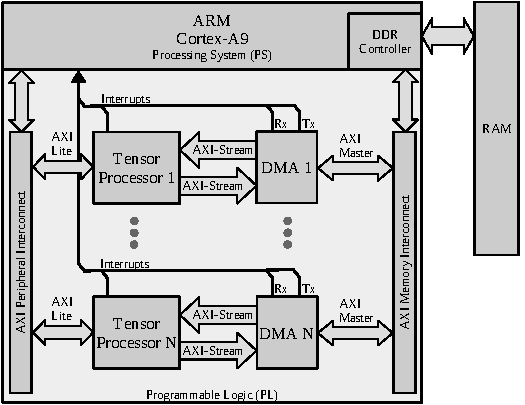
\includegraphics[width=0.5\textwidth]{../figures/system_design.pdf}
	\caption{Base embedded system architecture.}
	\label{fig:system_architecture}
\end{figure}
\subsection{Tensor processor}
The TP is a dedicated hardware module to compute tensor operations. The hardware architecture is described in \fig{fig:accelerator}. This architecture implements high performance communication with AXI-Stream, direct CPU communication with AXI-Lite, and on-chip storage utilizing BRAM. This hardware architecture is implemented with high-level synthesis (HLS). The tensor operations are implemented based on the C++ TensorFlow Lite micro kernels.

The TP is an extensible hardware module that executes low-level tensor operations. In this paper, we focus on the \emph{Conv2D} tensor operation that computes 2D convolution layers.

\begin{figure}[t!]
	\centering
	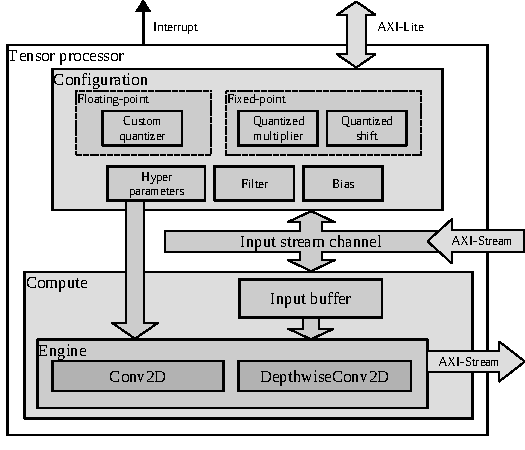
\includegraphics[width=0.5\textwidth]{../figures/accelerator.pdf}
	\caption{Hardware architecture of the proposed tensor processor.}
	\label{fig:accelerator}
\end{figure}
\subsubsection{\textbf{Modes of operation}}
The TP has two modes of operation: \emph{configuration} and \emph{execution}.
\begin{itemize}
	\item In \emph{configuration} mode, the TP receives the tensor operation ID for \emph{Conv2D} and hyperparameters: stride, dilation, padding, offset, activation, depth-multiplier, input shape, filter shape, bias shape, and output shape. Afterwards, the TP receives filter and bias tensors, which are locally stored in BRAM. The filter and bias tensors are transferred with standard FP representation. The TP extracts the 6-bit format for local on-chip storage.
	
	\item In \emph{execution} mode, the TP executes the tensor operation according to the hyperparameters given in the configuration mode. During execution, the input and output tensors are moved from/to the DDR memory via DMA.
\end{itemize}
\subsubsection{\textbf{Dot-product with hybrid floating-point}}
\label{sec:dot_product}
We implement the floating-point computation adopting the dot-product with hybrid custom floating-point\cite{nevarez2021accelerating}. The hardware dot-product is illustrated in \Fig{fig:dot_product}. This approach: (1) denormalizes input values, (2) executes computation with integer format for exponent and mantissa, and finally, (3) it normalizes the result into IEEE 754 format, see \Fig{fig:dot_product_hybrid}. 

Rather than a parallelized structure, this is a pipelined hardware design suitable for resource-limited devices. The latency in clock cycles of this hardware module is defined by \equ{eq:dot_custom_float_latency}, where $N$ is the vector length. The latency equations are obtained from the general pipelined hardware latency formula: $L=\left(N-1\right)II+IL$, where $II$ is the initiation interval (\fig{fig:dot_product_hybrid}(a)), and $IL$ is the iteration latency (\fig{fig:dot_product_hybrid}(b)). Both $II$ and $IL$ are obtained from the high-level synthesis results. Both the exponent and mantissa bit widths of the filter and bias buffers are set to a 4-bit exponent and a 1-bit mantissa (E4M1), which corresponds to float6 quantization. The 1-bit mantissa enables low-power multiply-accumulate (MAC) implementations by reducing the mantissa multiplication to a flag operation. This approach reduces energy consumption and resource utilization.

\begin{eqnarray} \label{eq:dot_custom_float_latency}
L_{hf}=N+7
\end{eqnarray}

The Infinity and NaN special cases are not considered in this design since are not expected in ANN computation. For the FP subnormal case, the element-wise multiplication skips when having a zero entry and applies approximation when having subnormal mantissas. The 1-bit mantissa has one subnormal case, which is handled as a normalized case. This simplifies the hardware design.

The approximation error is defined by the difference between \Equ{eq:float} and \Equ{eq:float_subnorm} when $E=0$ and $M=2^{-1}$, which defines the error as $e=2^{-B-1}$. From \Equ{eq:float_bias} with $E_size=4$, we have $B=7$. Hence, $e=3.9\mathrm{e}{-3}$. This error is produced when having the subnormal case $E=0$ and $M=2^{-1}$, which corresponds to the value $\pm7.8\mathrm{e}{-3}$ deviated to $\pm1.17\mathrm{e}{-3}$. This approximation is allowed base on the intrinsic error tolerance of neural networks\cite{du2014leveraging}.

\begin{figure}[t!]
	\centering
	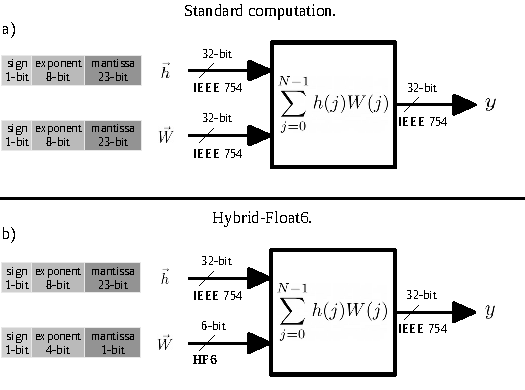
\includegraphics[width=0.5\textwidth]{../figures/dot-product_unit.pdf}
	\caption{Dot-product hardware module with (a) standard floating-point and (b) Hybrid-Float6.}
	\label{fig:dot_product}
\end{figure}

\begin{figure}[t!]
	\centering
	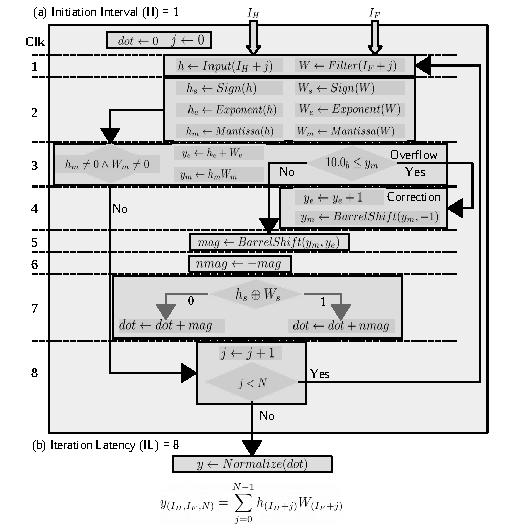
\includegraphics[width=0.5\textwidth]{../figures/dot_product_hybrid.pdf}
	\caption{Pipelined hardware module for vector dot-product with hybrid custom floating-point, (a) exhibits the initiation interval of 1 clock cycle, and (b) presents
		the iteration latency of 8 clock cycles. $I_H$ and $I_F$ represent the input and filter buffer indexes, respectively.}
	\label{fig:dot_product_hybrid}
\end{figure}

\subsubsection{\textbf{On-chip memory utilization}}
\label{sec:memory_utilization}
The total on-chip memory utilization on the TP is defined by \Equ{eq:tp_memory}, where $TP_B$ and $V_{M}$ represent the tensor buffers and local variables (memory) required for the design, respectively. \Equ{eq:tp_memory_buffer} defines the tensor buffers, where $Input_{M}$ is the \emph{input buffer}, $Filter_{M}$ is the \emph{filter buffer}, $Bias_{M}$ is the \emph{bias buffer}. The on-chip memory buffers are defined in bits. \fig{fig:accelerator_buffers} illustrates the convolution operation utilizing the on-chip memory buffers.
\begin{figure}[t!]
	\centering
	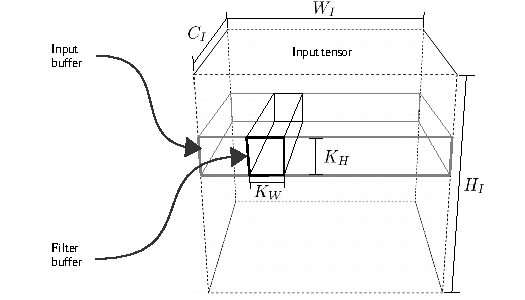
\includegraphics[width=0.5\textwidth]{../figures/accelerator_buffers.pdf}
	\caption{Design parameters for on-chip memory buffers on the TP.}
	\label{fig:accelerator_buffers}
\end{figure}
\begin{eqnarray} \label{eq:tp_memory}
TP_{M}=TP_B+V_{M}
\end{eqnarray}
\begin{eqnarray} \label{eq:tp_memory_buffer}
TP_{B}=Input_{M}+Filter_{M}+Bias_{M}
\end{eqnarray}

The memory utilization of \emph{input buffer} is defined by \Equ{eq:input_memory}, where $K_{H}$ is the height of the convolution kernel, $W_{I}$ is the width of the input tensor, $C_{I}$ is the number of input channels, and $BitSize_{I}$ is the bit size of input tensor.
\begin{eqnarray} \label{eq:input_memory}
Input_{M}=K_{H}W_{I}C_{I}BitSize_{I}
\end{eqnarray}

The memory utilization of \emph{filter buffer} is defined by \Equ{eq:filter_memory}, where $K_{W}$ and $K_{H}$ are the width and height of the convolution kernel, respectively; $C_{I}$ and $C_{O}$ are the number of input and output channels, respectively; and $BitSize_{F}$ is the bit size of filter values.
\begin{eqnarray} \label{eq:filter_memory}
Filter_{M}=C_{I}K_{W}K_{H}C_{O}BitSize_{F}
\end{eqnarray}

The memory utilization of \emph{bias buffer} is defined by \Equ{eq:bias_memory}, where $C_{O}$ is the number of output channels, and $BitSize_{B}$ is the bit size of bias values.
\begin{eqnarray} \label{eq:bias_memory}
Bias_{M}=C_{O}BitSize_{B}
\end{eqnarray}

As a design trade-off, \Equ{eq:channel_in_memory} defines the capacity of output channels based on the given design parameters. The total on-chip memory $TP_{M}$ determines the TP capacity.
\begin{eqnarray} \label{eq:channel_in_memory}
C_{O}=\frac{TP_{M}-V_{M}-K_{H}W_{I}C_{I}BitSize_{I}}{C_{I}K_{W}K_{H}BitSize_{F}+BitSize_{B}}
\end{eqnarray}

The floating-point formats implemented in the TP are defined by $BitSize_F$, $BitSize_B$ and $BitSize_I$. The HF6 defines 6-bit for $BitSize_F$ and $BitSize_B$, and 32-bit for $BitSize_I$. These are design parameters defined before hardware synthesis. This allows fine control of BRAM utilization, which is suitable for resource-limited devices.

\subsection{Training Method}
The models are trained and quantized in separate stages.
\subsubsection{Training with Iterative Early Stop}
To achieve better performance on CNN-regression models, we implement a training procedure with iterative early stop cycle. This allows to reach better local minima. This is a four steps process: (1) a base model is obtained with an initial training, (2) the base model is iteratively re-trained to search for better local minima, (3) in case of a better local minimum, the base model is updated/saved and used for subsequent re-training iterations, (4) the training cycle stops automatically with a given patience for unsatisfactory search iterations. See \Algo{alg:training}. This method minimizes the MSE.

\REVIEW{Talk about the moving averages.}

\subsubsection{Quantization Aware Training}
The quantization aware training (QAT) method is integrated into the training process, this operates after each mini-batch update. The quantization is applied on the trainable parameters of convolution layers. This method is implemented as a callback function in the TensorFlow/Keras framework, see \Algo{alg:quantization_integration}.

The quantization method uses rounding strategy to reduce the FP representation. This maps the full precision FP values to the closest representable 6-bit FP values, see \Algo{alg:quantize_training}. This method quantizes the filter and bias tensors of the convolution layers. We have observed that the exponent bit size plays a more predominant influence on the model accuracy than the mantissa bit size. In \cite{lai2017deep}, Lai et al. demonstrated that 4-bit exponent is adequate and consistent across different networks (SqueezeNet, AlexNet, GoogLeNet, VGG-16). In this work, we investigate 4-bit exponent and 1-bit mantissa.

\begin{algorithm}[h!]
	\label{alg:training}
	\caption{Training with iterative early stop cycle.}
	\begin{algorithmic}
		\SetAlgoLined
		\renewcommand{\algorithmicrequire}{\textbf{input:}}
		\renewcommand{\algorithmicensure}{\textbf{output:}}
		\REQUIRE $MODEL$ as the input model.
		\REQUIRE $D_{train}$ as the training data set.
		\REQUIRE $D_{val}$ as the validation data set.
		\REQUIRE $N_{I}$ as the stop patience for iterative training cycle.
		\REQUIRE $N_{E}$ as the early stop patience (epochs) for training.
		\REQUIRE $B_{size}$ as the mini-batch size.
		\ENSURE $MODEL$ as the full-precision output model.
		\STATE $Train(MODEL, D_{train}, D_{val}, N_{E}, B_{size})$
		\STATE $mse_i \gets Evaluate(MODEL, D_{val})$ // Benchmark
		\STATE $n_i \gets 0$
		\WHILE {$n_I<N_I$}
		\STATE // Iterative early stop cycle
		\STATE $Train(MODEL, D_{train}, D_{val}, N_{E}, B_{size})$
		\STATE $mse_v \gets Evaluate(MODEL, D_{val})$
		\IF{$mse_v < mse_i$}
			\STATE $Update(MODEL)$
			\STATE $mse_i \gets mse_v$
		\ELSE
			\STATE $MODEL  \gets LoadPreviousModel()$
			\STATE $n_I \gets n_I + 1$
		\ENDIF
		\ENDWHILE
	\end{algorithmic}
\end{algorithm}


\begin{algorithm}[h!]
	\label{alg:quantization_integration}
	\caption{Quantization aware training.}
	\begin{algorithmic}
		\SetAlgoLined
		\renewcommand{\algorithmicrequire}{\textbf{input:}}
		\renewcommand{\algorithmicensure}{\textbf{output:}}
		\REQUIRE $MODEL$ as the full-precision input model.
		\REQUIRE $E_{size}$ as the target exponent bits size.
		\REQUIRE $M_{size}$ as the target mantissa bits size.
		\REQUIRE $D_{train}$ as the training data set.
		\REQUIRE $D_{val}$ as the validation data set.
		\REQUIRE $N_{ep}$ as the number of epochs.
		\REQUIRE $B_{size}$ as the mini-batch size.
		\ENSURE $MODEL$ as the quantized output model.
		\STATE $MODEL \gets Quantize(MODEL,E_{size}, M_{size})$
		\STATE $mse_i \gets Evaluate(MODEL, D_{val})$ // Benchmark
		\STATE $Train(MODEL, D_{train}, D_{val}, N_{ep}, B_{size})$
		\STATE
		\STATE \bf{OnMiniBatchUpdate\_Callback():}
		\STATE $MODEL \gets Quantize(MODEL,E_{size}, M_{size})$
		\IF {$1<epoch$}
		\STATE // Update model after first epoch
		\STATE $mse_v \gets Evaluate(MODEL, D_{val})$
		\IF{$mse_v < mse_i$}
		\STATE $Update(MODEL)$
		\STATE $mse_i \gets mse_v$
		\ENDIF
		\ENDIF
	\end{algorithmic}
\end{algorithm}

\begin{algorithm}[h!]
	\label{alg:quantize_training}
	\caption{Custom floating-point quantization.}
	\begin{algorithmic}
		\SetAlgoLined
		\renewcommand{\algorithmicrequire}{\textbf{input:}}
		\renewcommand{\algorithmicensure}{\textbf{output:}}
		\REQUIRE $MODEL$ as the CNN.
		\REQUIRE $E_{size}$ as the target exponent bit size.
		\REQUIRE $M_{size}$ as the target mantissa bits size.
		\REQUIRE $STDM_{size}$ as the IEEE 754 mantissa bit size.
		\ENSURE $MODEL$ as the quantized CNN.
		\FOR {$layer$ in $MODEL$}
		\IF {$layer$ is $Conv2D$ or $SeparableConv2D$}
		\STATE $filter, bias \gets GetWeights(layer)$
		\FOR {$x$ in $filter$ and $bias$}
			\STATE $sign \gets GetSign(x)$
			\STATE $exp \gets GetExponent(x)$
			\STATE $fullexp \gets 2^{E_{size}-1}-1$ // Get full range value
			\STATE $cman \gets GetCustomMantissa(x, M_{size})$
			\STATE $leftman \gets GetLeftoverMantissa(x, M_{size})$
			\IF {$exp <-fullexp$}
				\STATE$x\gets0$
			\ELSIF{$exp > fullexp$}
				\STATE$x\gets (-1)^{sign}\cdot2^{fullexp}\cdot(1+(1-2^{-M{size}}))$
			\ELSE
				\IF {$2^{STDM_{size}-M_{size}-1}-1<leftman$}
					\STATE $cman \gets cman+1$ // Above halfway
					\IF{$2^{M_{size}}-1<cman$}
					\STATE $cman \gets 0$ // Correct mantissa overflow
					\STATE $exp \gets exp + 1$
					\ENDIF
				\ENDIF
				\STATE // Build custom quantized floating-point value
				\STATE$x\gets (-1)^{sign}\cdot2^{exp}\cdot(1+cman\cdot2^{-M_{size}})$
			\ENDIF
		\ENDFOR
		\STATE $SetWeights(layer, filter, bias)$
		\ENDIF
		\ENDFOR
	\end{algorithmic}
\end{algorithm}
\begin{figure}[t!]
	\centering
	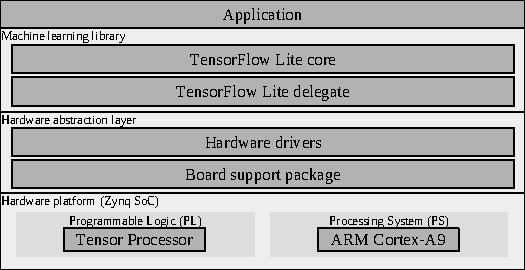
\includegraphics[width=0.5\textwidth]{../figures/sw_stack.pdf}
	\caption{Base embedded software architecture.}
	\label{fig:sw_stack}
\end{figure}
\subsection{Embedded software architecture}
The software architecture is a layered object-oriented application framework written in C++, see \fig{fig:sw_stack}. A description of the software layers is as follows:
\begin{itemize}
	\item \emph{Application}: As the highest level of abstraction, this software layer implements the application invoking the ML library.
	\item \emph{Machine learning library}: This layer consist of TensorFlow Lite for micro controllers. This offers a comprehensive high level API that allows ML inference. This provides delegate software interfaces for custom hardware accelerators.
	\item \emph{Hardware abstraction layer}: This layer consist of the hardware drivers to handle initialization and runtime operation of the TP and DMA.
\end{itemize}
\section{Experimental Results}
\label{sec:experimental_results}
In this section, we present experimental results using a low-power/low-cost sensor analytics application. As a use case, we present a CNN-regression model to predict x- y- coordinates of acoustic emissions based on piezoelectric vibrations. We compare quantitative and qualitative aspects of the analytics using floating-point 32-bit, fixed-point 8-bit, Hybrid-Logarithmic 6-bit, and Hybrid-Float6.

To demonstrate the proposed concept, we deploy the CNN model in the smallest Zynq SoC device for low-power inference. We compare the performance of the TP synthesized with standard FP (using Xilinx LogiCORE IPs) and Hybrid-Float6 design.

\subsection{Sensor Analytics Application}
The analytics model is designed to predict x- y- coordinates of acoustic emissions on a metal plate. The metal plate is in the presence of noise disturbance to simulate realistic conditions. In this subsection, we present the structure for experimental setup, data sets, and the CNN-regression model.

\subsubsection{Experimental Setup}
The experiment uses eight piezoelectric sensors (Vallen Systeme VS900) attached with magnetic holders on a metal plate (90 cm x 86.6 cm x 0.3 cm). The VS900 devices can operate either in active or passive mode. Six VS900 are used in passive mode as acoustic sensors and two in active mode to produce acoustic emissions. These acoustic emissions simulate anomalies on x- y- coordinates as well as the noise disturbance on the system. See \fig{fig:data_set}(a). To create data sets, the samples of acoustic emissions are labeled with their coordinates.

\subsubsection{Data Sets}
The data sets are recorded applying pulses on the metal plate, the x- y- coordinates of these pulses are used as labels. The pulses for training and validation data sets are shown in \fig{fig:data_set}(b) and \fig{fig:data_set}(c), respectively. The pulses for training and validation data sets are mutually exclusive, this exclusion is represented by the cross symbols in \fig{fig:data_set}(c). This creates a grid layout used to collect samples for the data sets. This grid is $10\times10$. This grid does not consider the four corners as they are used for magnetic holders.

\begin{figure}[t!]
	\centering
	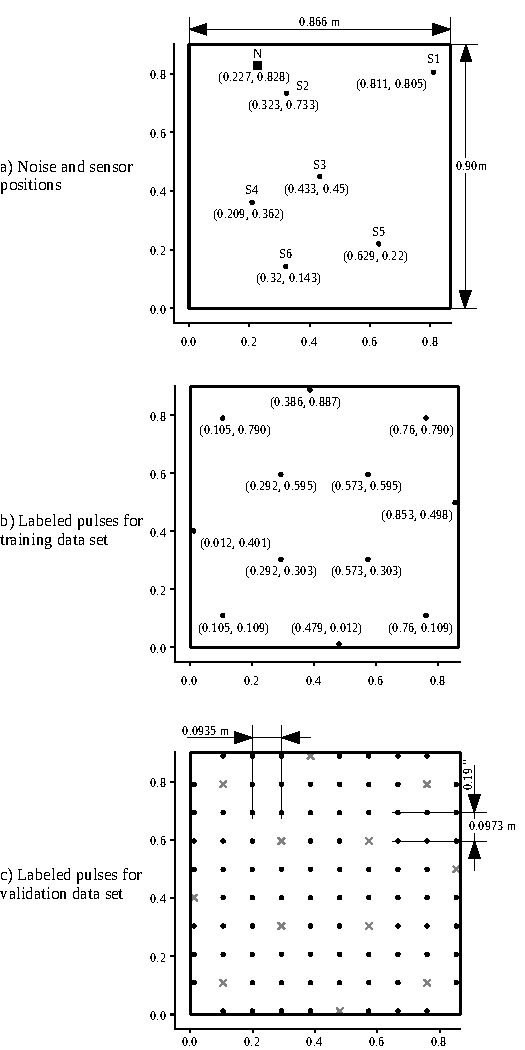
\includegraphics[width=\columnwidth]{../figures/histograms/data_set.pdf}
	\caption{Experimental setup for sensor analytics on structural health monitoring, all lengths are in meters (m).}
	\label{fig:data_set}
\end{figure}

In order to create reproducible acoustic emissions, we use 9-cycle sine pulse in a Hanning window with central frequency $f_\mathrm{c}$ (narrow-banded in the frequency domain). We assume guided Lamb waves based on the plate structure. The narrow-band behavior also reduces the dispersion of the acoustic emission waves~\cite{hannwindowsine}. The waveform can be expressed as a function of time $t$ as follows:

\begin{equation}
x_\mathrm{pulse}(t) = \frac{1}{2} \Big(1-\cos{\frac{f_\mathrm{c} t}{5}} \Big) A_0 \sin{f_\mathrm{c} t}.
\end{equation}

To generate the data sets, we use slightly different pulse amplitudes and frequencies for excitation. The pulse frequency $f_c$ is varied in 1 kHz steps between $\unit[300]{kHz}$ and $\unit[349]{kHz}$ and the amplitude $A_0$ is varied in $\unit[0.1]{V}$ steps between $\unit[2.6]{V}$ and $\unit[3.5]{V}$. This results in 500 different pulses for each of the excitation points.

The signals for labeled pulses and noise disturbance are generated by arbitrary waveform generators (AWGs). The sensor signals are recorded via a Vallen AMSY-6 measurement system with a resolution of 18 bits and a sampling rate of $f_\mathrm{S} =\unit[10]{MHz}$. The disturbance signal is gaussian noise with amplitudes between 0-3 V. This noise is applied via the piezoelectric device $N$ at $x=\unit[0.227]{m}$ and $y=\unit[0.828]{m}$, see \fig{fig:data_set}(a).

To obtain frequency components, the sampled pulses are converted into the frequency-time domain using the Short-Time Fourier Transform (STFT). This is calculated as follows~\cite{stft_lit}:

\begin{flalign}
\label{stft_eq2}
\mathcal{F}_{m,k}^\gamma= \sum_{n=0}^{N-1} x[n] \cdot \gamma^*[n-m\Delta M]\cdot \mathrm{e}^{\frac{-j 2 \pi k n }{N}}
\end{flalign}

Here $x[n]$ describes a discrete-time signal and $\gamma^*[n-m\Delta M]\cdot \mathrm{e}^{\frac{-j 2 \pi k n }{N}}$ the time- and frequency-shifted window function inside the considered interval $[0 , N-1]$. $\Delta M$ describes the time shift and $N$ the transformation window. Since only discrete frequencies and time points are considered, $m = 0,1,...,M-1$ is valid. For pictorial representation, the magnitude of the complex-valued STFT is employed in a spectrogram $\mathcal{S}_{m,k}$:

\begin{flalign}
\label{stft_eq3}
\mathcal{S}_{m,k}= \left|\mathcal{F}_{m,k}^\gamma\right|^2 = \left|\sum_{n=0}^{N-1} x[n] \cdot \gamma^*[n-m\Delta M]\cdot \mathrm{e}^{\frac{-j 2 \pi k n }{N}} \right|^2
\end{flalign}

In addition, these spectrograms are scaled in decibels. The spectrogram in decibels $\mathcal{S}_{m,k,\mathrm{dB}}$ results in $\mathcal{S}_{m,k,\mathrm{dB}}= 20 \cdot \mathrm{log}_{10}(\mathcal{S}_{m,k})$. For the conversion of the data, we use a signal length of 400 \textmu s (75 \textmu s pretrigger and 325 \textmu s post trigger). Thus, the arrival times of the pulses are included in the spectrogram for all channels and labeled positions. We use a Blackman window function~\cite{blackman_window}, a Fast Fourier Transform (FFT) length of 32 samples, and an overlap of 8 samples. The spectrograms are calculated for frequencies in the range of 100 kHz to 500 kHz. This results in a spectrogram size of 8x16 (8 frequency bins, 16 time values).

In order to generate larger data sets, we create four further variants with time shifts of 15 \textmu s/ 30 \textmu s/ 45 \textmu s/ 60 \textmu s. Subsequently, all spectrograms are converted to grayscale with scaling between -100dB and -40dB, see \fig{fig:spectrograms}.

In overall, the data set has a size of 1,440,000 images. This is the result of 500 (pulses) $\cdot$ 5 (spectrograms) $\cdot$ 6 (listening sensors) $\cdot$ 96 (excitation points).

\begin{figure}[t!]
	\centering
	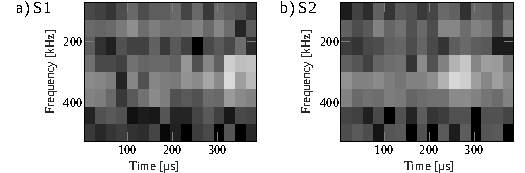
\includegraphics[width=\columnwidth]{../figures/histograms/spectrograms.pdf}
	\caption{Spectrograms of sensors $S_1, S_2$ converted to grayscale for pulses at $x =0.105$ m, $y = 0.109$ m with noise disturbance.}
	\label{fig:spectrograms}
\end{figure}

\subsubsection{CNN-Regression Model}
The data analytics is implemented with a CNN-regression model, see \fig{fig:model}. The structure of the model is described below:

\begin{enumerate}[label=\alph*)]
\item Input tensor. This is composed of spectrograms from the sensor signals. The tensor shape is defined by $S \times T \times F$, where $S$ is the number of sensors, and $T \times F$ is the time-frequency resolution of the spectrograms, see \fig{fig:model}(a).

\item Feature extraction. This is composed of three blocks of convolution, batch normalization, and max-pooling layers, see \fig{fig:model}(b). The number of channels in the convolution layers are defined by the hyper-parameters $A$, $B$, and $C$.

\item Regression function. This is an arbitrary function implemented with two fully connected layers and an output layer with linear activation, see \fig{fig:model}(c).
\end{enumerate}


\begin{figure}[t!]
	\centering
	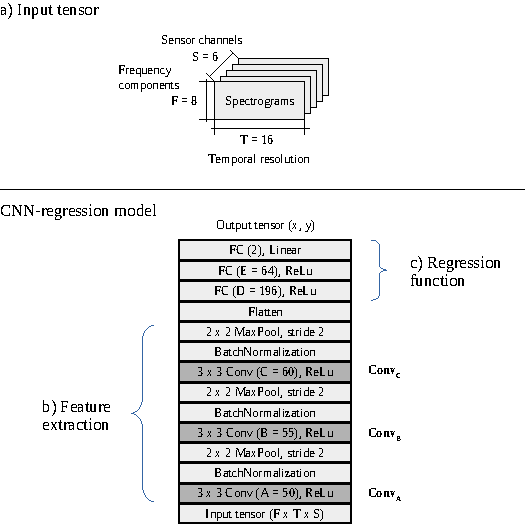
\includegraphics[width=\columnwidth]{../figures/models.pdf}
	\caption{CNN-regression model for sensor analytics.}
	\label{fig:model}
\end{figure}


\subsection{Training}
\subsubsection{Base Model}
The model in \fig{fig:model} is trained using Adam algorithm with iterative search. The Adam optimizer is configured with the default settings presented in \cite{kingma2014adam}: $\alpha = 0.001$, $\beta_1 = 0.9$, $\beta_2 = 0.999$, and $\epsilon = 1\mathrm{e}{-8}$. The training cycle patience is 10 iterations, the optimizer is executed with early stop patience of 10 epochs, and mini-batch size of 512 samples. This is applied using the method described in \Algo{alg:training} with $N_I = 10$, $N_E=10$, $B_{size}=512$.

The training results are illustrated in \fig{fig:optimization}(a). In this optimization, the initial and the final models achieve $MSE=\unit[0.0135]{m^2}$ and $MSE=\unit[0.0122]{m^2}$, respectively. The $MSE$ is calculated with the Euclidean distance (loss) between the expected and the predicted coordinates. The initial model is obtained at the first early stop (after 10 epochs). In each stop, the moving averages of the Adam optimizer get re-initialized. This facilitates searching for better local minima. The model gets saved/updated when finding a better minimum.

\begin{figure}[h!]
	\centering
	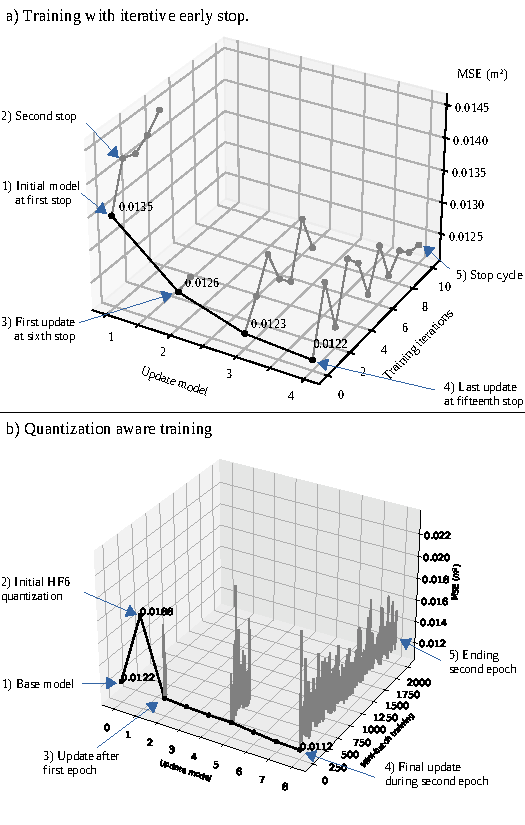
\includegraphics[width=\columnwidth]{../figures/histograms/training_and_quantization.pdf}
	\caption{Training results.}
	\label{fig:optimization}
\end{figure}

The final model achieves $MSE=\unit[0.0122]{m^2}$, which corresponds to $MAE=\unit[0.0955]{m}$. See \fig{fig:model_evaluation}(a). In total, the training takes 379 epochs in 25 cycle-search iterations. The first search takes 43 epochs for the initial model and subsequent search iterations take an average of 14 epochs. The total time is 53 minutes using a PC with AMD Ryzen 5 5600H and NVIDIA GeForce RTX 3050.

\begin{figure}[h!]
	\centering
	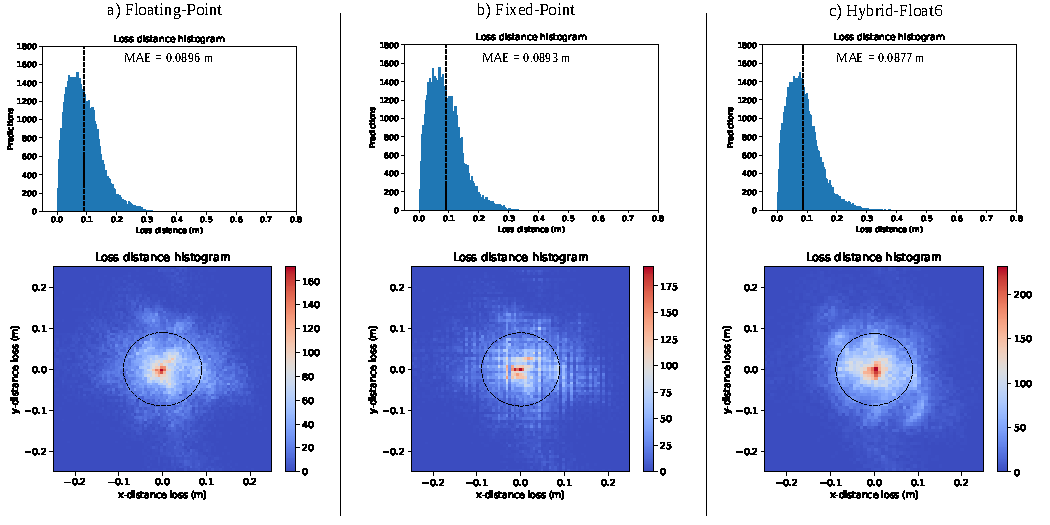
\includegraphics[width=\columnwidth]{../figures/histograms/model_evaluation.pdf}
	\caption{Performance of the model with different data representations.}
	\label{fig:model_evaluation}
\end{figure}

\subsubsection{TensorFlow Lite 8-bit Quantization}
This optimization method converts filter and bias tensors as well as activation maps to 8-bit integer representation, this allows inference using integer-only arithmetic\cite{hannwindowsine}. In this research, this quantization is applied only to the convolution layers as they are the compute bound operations. Other layers employ 32-bit FP representation.

In the compute graph, the imput and output feature maps are glued with linear quantization at the input and output of the \emph{Conv2D} operations.

The base model is quantized using the TensorFlow Lite library with integer-only quantization on the \emph{Conv2D} tensor operations. The filter and bias tensors are represented by 8-bit and 32-bit signed integers, respectively. The input and output activation maps are represented by 8-bit signed integer. The TensorFlow quantization includes two additional vectors (output-multiplier and output-shift coefficients), these two vectors are the same shape as the bias vector with 32-bit integer representation.

This model achieves $MSE=\unit[0.0126]{m^2}$ and $MAE=\unit[0.0992]{m}$. See \fig{fig:model_evaluation}(b). The MAE increases 5.1\% of the base model. We attribute this degradation to the 8-bit quantization on the \emph{Conv2D} layers.

\subsubsection{Inference of non-quantized models on HF6 hardware}
We explore the inference of the base model without quantization on the HF6 hardware. See \fig{fig:model_evaluation}(c). This obtains $MSE=\unit[0.0188]{m^2}$ and $MAE=\unit[0.1232]{m}$. The MAE increases 29.5\% of the base model. We attribute this degradation to the rounding errors of non-quantized filters and bias in \emph{Conv2D} layers.

\subsubsection{Quantization-Aware Training for HF6 hardware}
The QAT is a post-training optimization. We run the QAT during two epochs with mini-batch size of 10 samples. This a custom floating-point quantization  targeting the HF6 format: 4-bit exponent and 1-bit mantissa. This is applied to filter and bias tensors of \emph{Conv2D} layers. This method is described in \Algo{alg:quantization_integration} with $N_{ep}=2$, $B_{size}=10$, $E_{size}=4$, $M_{size}=1$. The optimization results are illustrated in \fig{fig:optimization}(b).

The resulting model achieves $MSE=\unit[0.0112]{m^2}$ and $MAE=\unit[0.0919]{m}$. This corresponds to an error reduction of 8.2\% and 3.77\%, respectively. We attribute this improvement to the regularization effect. See \fig{fig:model_evaluation}(d). The QAT time is 185 minutes.


\subsubsection{Quantization-Aware Training for Hybrid-Logarithmic 6-bit}
For the sake of quality comparison with logarithmic quantization, we generate the model with 6-bit logarithmic representation on trainable parameters of convolution layers. See \fig{fig:floating}(e). This quantization matches the bit size of HF6. The filter and bias tensors of \emph{Conv2D} layers are quantized with the 6-bit logarithmic format: 1-bit sign, 5-bit signed exponent, and 0-bit mantissa. This is applied using the method described in \Algo{alg:quantization_integration} with $N_{ep}=2$, $B_{size}=10$, $E_{size}=5$, $M_{size}=0$.

The model achieves $MSE=\unit[0.0123]{m^2}$ and $MAE=\unit[0.0968]{m}$, which correspond to an error increase of 0.82\% and 1.36\%, respectively. We attribute this degradation to the 6-bit logarithmic quantization. See \fig{fig:model_evaluation}(e).

A summary of improvement-degradation of MSE and MAE with different data representations is presented in \fig{fig:model_evaluation}(f).

\subsection{Hardware Design Exploration}
The proposed hardware/software co-design is demonstrated on the Zynq-7007S system-on-chip (SoC) on the MiniZed development board. This SoC integrates a single ARM Cortex-A9 processing system (PS) and a programmable logic (PL) equivalent to Xilinx Artix-7 (FPGA) in a single chip \cite{xilinx2015zynq}. The Zynq-7007S SoC architecture maps the custom logic and software in the PL and PS, respectively.

In this platform, we implement the proposed hardware/software architecture to deploy the sensor analytics application. The desired model is converted to TensorFlow Lite (floating-point) and deployed on the embedded software as a hex dump in a C array. The Zynq-7007S SoC executes inference with TensorFlow Lite on the PS. The computational workload of convolution layers is delegated to the dedicated hardware.

\subsubsection{Benchmark on Embedded CPU}
First, we explore the performance of the embedded CPU for inference without hardware acceleration. In this case, TensorFlow Lite creates the CNN model as a sequential compute graph executing all computation on the CPU (ARM Cortex-A9) at $\unit[666]{MHz}$ and power dissipation of $\unit[1,187]{W}$.

The compute performance and run-time inference of the CPU are shown in \Tab{tab:performance}(a) and \fig{fig:runtime}(a), respectively.

\subsubsection{Benchmark on Tensor Processor Synthesized with Xilinx LogiCORE IP for Floating-Point Computation}
For this design, we implement the TP with standard FP hardware prior synthesis. The design parameters for the maximum required accelerator on-chip size are:
\begin{itemize}
	\item Max convolution kernel size: $K_W = K_H = 3$.
	\item Max input tensor width: $W_I = 16$.
	\item Max input and output channels: $C_I = 55$, $C_O = 60$.
	\item Filter and bias bit size: $BitSize_F=BitSize_B=32$.
	\item Input tensor bit size: $BitSize_I=32$.
\end{itemize}

Using equations from Section \ref{sec:memory_utilization}, the on-chip memory buffer utilization are $Input_M=84,480$b, $Filter_M=950,400$b, and $Bias_M=1,920$b. Hence, the required on-chip memory buffer size is $TP_B=1,036,800$b.

The post-implementation resource utilization and power dissipation are presented in \Tab{tab:resource_utilization}(a). The complete hardware platform utilizes 83\% of BRAM, this includes the on-chip memory requirements of the TP, DMA, and AXI interconnects. The total available on-chip memory (BRAM) on the Zynq-7007S SoC is $\unit[1.8]{Mb}$. After hardware syntheses, the estimated power dissipation of the TP is $\unit[85]{mW}$ at $\unit[200]{MHz}$ (this estimation is provided by Xilinx Vivado).

\begin{table}[!h]\centering
	\caption{Resource utilization and power dissipation on the Zynq-7007S SoC.}\label{tab:resource_utilization}
	\scriptsize
	\begin{tabular}{lrrrrrr}\toprule
		\multirow{2}{*}{\textbf{TP engine}} &\multicolumn{4}{c}{\textbf{Post-implementation resource utilization}} &\multirow{2}{*}{\textbf{Power (W)}} \\\cmidrule{2-5}
		&\textbf{LUT} &\textbf{FF} &\textbf{DSP} &\textbf{BRAM 36Kb} & \\\midrule
		\multirow{2}{*}{(a) Floating-Point} &5,578 &8,942 &23 &41.5 &\multirow{2}{*}{1.429} \\
		&39\% &31\% &35\% &\textbf{83\%} & \\
		\multirow{2}{*}{(b) Hybrid-Float6} &7,313 &10,330 &20 &15 &\multirow{2}{*}{1.424} \\
		&51\% &36\% &30\% &\textbf{30\%} & \\
		\bottomrule
	\end{tabular}
\end{table}

The compute performance and inference schedule of the model on this hardware implementation are shown in \Tab{tab:performance}(b) and \fig{fig:runtime}(b), respectively. During run-time, TensorFlow Lite delegates computation to the TP as dedicated hardware for \emph{Conv2D} tensor operations.

The implementation of the dot-product with standard FP engine (IEEE 754 arithmetic) utilizes proprietary multiplier and adder FP operator cores. Vivado HLS implements FP arithmetic operations by mapping them onto Xilinx LogiCORE IP cores, these FP operator cores are instantiated in the resultant RTL \cite{hrica2012floating}. In this case, the implementation of the dot-product with the standard FP computation reuses the multiplier and adder cores in different compute sections of the TP. The post-implementation resource utilization and power dissipation of the individual floating-point operator cores are shown in \Tab{tab:LogiCORE}.

\begin{table}[!t]\centering
	\caption{Compute performance of the CPU and TP on each Conv2D tensor operation. This table presents: tensor operation, computational cost in mega floating-point operations (MFLOP), latency, throughput, power efficiency, and estimated energy consumption as the energy delay product (EDP).}\label{tab:performance}
	\scriptsize
	\begin{tabular}{lrrrrrr}\toprule
		\textbf{Operation} &\textbf{MFLOP} &\textbf{t (ms)} &\textbf{MFLOP/s} &\textbf{MFLOP/s/W} &\textbf{EDP (mJ)} \\\midrule
		& &\multicolumn{4}{l}{\textbf{a) CPU (ARM Cortex-A9) @666MHz, 1.187 W}} \\
		Conv\textsubscript{A} &0.691 &112.24 &6.16 &5.19 &133.23 \\
		Conv\textsubscript{B} &1.584 &213.13 &7.43 &6.26 &252.99 \\
		Conv\textsubscript{C} &0.475 &46.59 &10.20 &8.59 &55.31 \\
		& &\multicolumn{4}{l}{\textbf{b) TP (Floating-Point engine) @200MHz, 85 mW}} \\
		Conv\textsubscript{A} &0.691 &12.49 &55.34 &651.11 &1.06 \\
		Conv\textsubscript{B} &1.584 &16.39 &96.66 &1,137.20 &1.39 \\
		Conv\textsubscript{C} &0.475 &3.59 &132.44 &1,558.13 &0.30 \\
		& &\multicolumn{4}{l}{\textbf{c) TP (Hybrid-Float6 engine) @200MHz, 84 mW}} \\
		Conv\textsubscript{A} &0.691 &6.92 &99.81 &1,188.24 &0.58 \\
		Conv\textsubscript{B} &1.584 &4.41 &358.94 &4,273.09 &0.37 \\
		Conv\textsubscript{C} &0.475 &0.99 &482.44 &5,743.29 &0.08 \\
		\bottomrule
	\end{tabular}
\end{table}

\begin{figure}[t!]
	\centering
	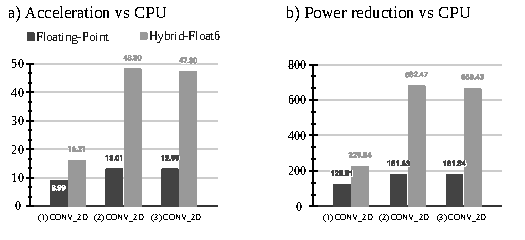
\includegraphics[width=1\columnwidth]{../figures/power_breakdown/acceleration_power_reduction.pdf}
	\caption{Inference acceleration and power reduction on the TP with floating-point and HF6 vs. CPU on the Zynq-7007S SoC.}
	\label{fig:acceleration}
\end{figure}


\begin{table}[!h]\centering
	\caption{Resource utilization and power dissipation of individual multiplier and adder floating-point (IEEE 754) operator cores (Xilinx LogiCORE IP).}\label{tab:LogiCORE}
	\scriptsize
	\begin{tabular}{lrrrrrr}\toprule
		\textbf{Core operation} &\textbf{DSP} &\textbf{FF} &\textbf{LUT} &\textbf{Latency (clk)} &\textbf{Power (mW)} \\\midrule
		Multiplier &3 &151 &325 &4 &7 \\
		Adder &2 &324 &424 &8 &6 \\
		\bottomrule
	\end{tabular}
\end{table}



\subsubsection{Tensor Processor Synthesized with Hybrid-Float6 Hardware Architecture}
To demonstrate the proposed design, the TP with HF6 hardware reuses the standard FP design parameters with the following variation for the 6-bit representation in filter and bias: $BitSize_F=BitSize_B=6$.

Using equations from Section \ref{sec:memory_utilization}, the on-chip memory requirements for the hardware accelerator are $Input_M=\unit[84,480]{b}$, $Filter_M=\unit[178,200]{b}$, $Bias_M=\unit[360]{b}$. Hence, the required on-chip memory buffer size is $TP_B=\unit[263,040]{b}$.

The post-implementation resource utilization and power dissipation are presented in \Tab{tab:resource_utilization}(b). The complete hardware platform utilizes 30\% of BRAM, this includes the on-chip memory requirements of the TP, DMA, and AXI interconnects. The estimated power dissipation of the TP is $\unit[84]{mW}$ at $\unit[200]{MHz}$ (this estimation is provided by Xilinx Vivado).

The compute performance and inference schedule of the model on this hardware implementation are shown in \Tab{tab:performance}(c) and \fig{fig:runtime}(c), respectively. \Fig{fig:acceleration} presents a comparison of the acceleration and the reduction of power dissipation between standard FP and HF6 hardware implementations.

This deployment does not require model treatment for hardware compatibility. For backward compatibility, the 6-bit FP representation is wrapped into the standard FP. The dedicated hardware design extracts the 6-bit format automatically to perform computation.

\begin{figure}[t!]
	\centering
	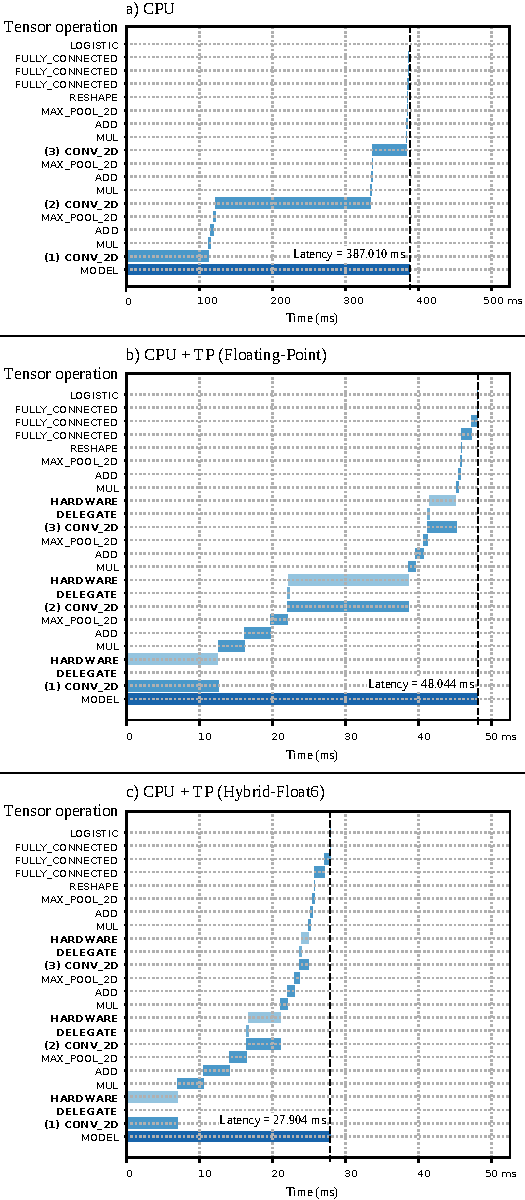
\includegraphics[width=1\columnwidth]{../figures/runtime/runtime.pdf}
	\caption{Run-time inference of TensorFlow Lite on the Zynq-7007S SoC. (a) CPU ARM Cortex-A9 at $\unit[666]{MHz}$, (b) cooperative CPU + TP with floating-point Xilinx LogiCORE IP at $\unit[200]{MHz}$, and (c) cooperative CPU + TP with Hybrid-Float6 at $\unit[200]{MHz}$.}
	\label{fig:runtime}
\end{figure}

\subsection{Discussion}
\subsubsection{Training and Quantization}
The training with iterative early stop obtains a model with enhanced accuracy than standard early stop. This method iteratively resets the moving averages of Adam's optimizer, which helps to iteratively search for better local minima. This iterative search is suitable for models with low computational cost.

The TensorFlow Lite 8-bit quantization preserves the overall model accuracy. In some cases, the associated regularization effect can improve the accuracy. However, the error distribution in CNN linear regressions gets slightly degraded. In particular, 8-bit quantized output layers incur in discrete-degradation patterns, \fig{fig:2d_error_distribtion}(b) shows this effect on three different models. Vertical and horizontal patterns appear in the error distribution of 8-bit fixed-point quantization. We attribute this effect to the 8-bit resolution in the activation maps. In the case of HF6 quantization, the activation maps are represented by floating-point preventing this degradation.

The proposed 6-bit FP representation (E4M1) improves latency, hardware area, and power dissipation, while preserving model accuracy. For comparison, in our application, this number format produces better results than the 6-bit logarithmic representation (E5M0). This is demonstrated in \Fig{fig:model_evaluation}(d) and \Fig{fig:model_evaluation}(e).

In \cite{lai2017deep}, Lai et al. demonstrated that 4-bit exponent and X-bit mantissa preserves accuracy on SqueezeNet, AlexNet, GoogLeNet, and VGG-16. To contribute on this, we investigate 4-bit exponent and 1-bit mantissa to ALL-CNN-C \cite{springenberg2014striving}, this produces an accuracy degradation of 1.39\% and 0.11\% with QAT. While applying 6-bit logarithmic produces a degradation of 11.18\% and 7.22\% with QAT.

\begin{figure}[t!]
	\centering
	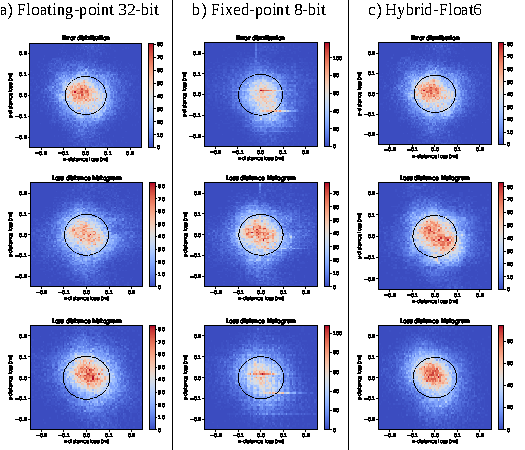
\includegraphics[width=1\columnwidth]{../figures/histograms/2D_error_distribtion.pdf}
	\caption{2D error distribution of three CNN-regression models.}
	\label{fig:2d_error_distribtion}
\end{figure}

\subsubsection{Implementation and Performance}
The proposed HF6 implementation reduces on-chip memory and DSP utilization while slightly increasing FF and LUT compared to the standard FP implementation. See \Tab{tab:resource_utilization} and \Fig{fig:resource_utilization}. We attribute this to the HF6 logic implementation using FF and LUT, while the FP logic implementation uses Xilinx LogiCORE IPs mainly with DSPs.

The compute performance of the CPU and TP on each convolution layer is presented in \Tab{tab:performance} and \fig{fig:acceleration}. 
The peak acceleration and power efficiency of the TP with standard FP (Xilinx LogiCORE IP) is $13\times$ and $1,558.13$ MFLOPS/s/W, respectively. While the peak acceleration and power efficiency of the TP with HF6 is $48.3\times$ and $5,743.29$ MFLOPS/s/W, respectively. The HF6 hardware demonstrates an improvement of $3.7\times$ in acceleration and power efficiency with respect to the standard FP hardware. See \Fig{fig:acceleration}.

The estimated power dissipation on the SoC is presented in \fig{fig:power}. This shows a very similar breakdown of power dissipation in both implementations. However, the energy efficiency is increased due to the reduced latency in HF6 hardware. A comparison of related work is presented in \Tab{tab:comparison}.

\begin{figure}[h!]
	\centering
	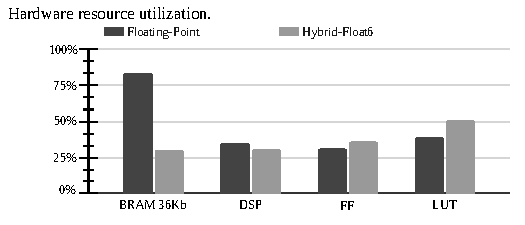
\includegraphics[width=1\columnwidth]{../figures/power_breakdown/resource_utilization.pdf}
	\caption{Hardware resource utilization on the Zynq-7007S SoC.}
	\label{fig:resource_utilization}
\end{figure}

\begin{figure}[h!]
	\centering
	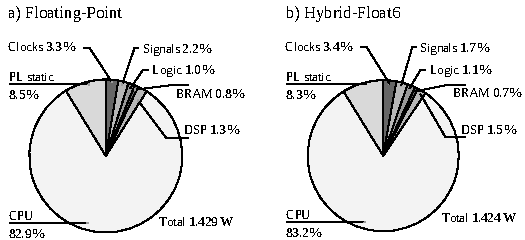
\includegraphics[width=1\columnwidth]{../figures/power_breakdown/power_breakdown.pdf}
	\caption{Estimated power dissipation on the Zynq-7007S SoC with PS at $\unit[666]{MHz}$ and PL at $\unit[200]{MHz}$.}
	\label{fig:power}
\end{figure}

The run-time inference of TensorFlow Lite on the SoC is illustrated in \Fig{fig:runtime}. This shows the convolution layers as the compute-bound operations. The proposed embedded platform is a cooperative system where the convolution operations are delegated to the dedicated hardware accelerator. The ARM CPU obtains a latency of $\unit[387]{ms}$ ($\unit[2.58]{FPS}$). The platform with standard FP hardware obtains a latency of $\unit[48]{ms}$ ($\unit[20.8]{FPS}$), while the implementation with HF6 obtains a latency of $\unit[27.9]{ms}$ ($\unit[35.84]{FPS}$). These represent an overall acceleration of $8\times$ and $13.87\times$ over the CPU, respectively.

This design facilitates ML compatibility/portability as the 6-bit FP is wrapped in the standard FP representation. The dedicated hardware design extracts the 6-bit format automatically and performs computation.

\subsubsection{SoC Design and Compatibility}
The proposed design is an alternative for high accuracy and low-power floating-point inference. The system runs as a cooperative hardware/software mechanism. This architecture delegates compute-bound tensor operations to a hardware accelerator.

The hybrid 32-bit FP and 6-bit FP quantization enables high quality of results and backward ML compatibility. Backwards ML compatibility gives portability from training to inference. This enables to run inference of HF6 quantized models on standard FP hardware and vise versa. The proposed HF6 architecture allows to compute inference of non-quantized floating-point ML models for rapid deployment; however, this will incur in accuracy degradation depending on the resilience of the model, see \Fig{fig:model_evaluation}(c).

\subsubsection{Future Work}
In this research, we foresee two lines of future work:
\begin{itemize}
\item \textbf{To reduce energy consumption.} Activation maps can be represented by Bfloat16 and 8-bit custom floating-point. This would reduce hardware resource utilization, memory footprint, and data transfer while preserving accuracy.

\item \textbf{To increase performance.} This implementation would require matching computational throughput with memory bandwidth using systolic arrays. This would replace the light-weight pipeline hardware design with a parallelized structure. This requires larger hardware area and energy consumption.
\end{itemize}

\begin{table*}[!t]\centering
	\caption{Comparison of hardware implementation with related work.}\label{tab:comparison}
	\scriptsize
	\begin{tabular}{lrrrrrr}\toprule
		Platform &Chunsheng Mei et al. \cite{mei2017200mhz} &Chen Wu et al. \cite{wu2021low} &BFP \cite{lian2019high} &Paolo Meloni et al. \cite{meloni2019cnn} &This work \\\midrule
		Device &XC7VX690T &XC7K325T &XC7VX690T &XC7Z007S &XC7Z007S \\
		Year &2017 &2019 &2019 &2019 &2022 \\
		Dev. kit cost &\$7,494 &\$1,299 &\$7,494 &\$89 &\$89 \\
		Format (activation/weight) &FP 16-bit &FP 8-bit / 8-bit &FP 16-bit / 8-bit &INT 16-bit &FP 32-bit / 6-bit \\
		Frequency (MHz) &200 &200 &200 &80 &200 \\
		Peak power efficiency (GFLOP/s/W) &18.72 &115.40 &82.88 &2.98 &5.74 \\
		Peak throughput (GFLOP/s) & 202.42 & 1086.8 & 760.83 &  10.62& 0.482\\
		Wall plug power (W) &10.81 &9.42 &9.18 &2.5 &2.3 \\
		BRAM 36Kb utilization &196.5 &234.5 &913 &44 &15 \\
		DSP utilization &1728 &768 &1027 &54 &20 \\
		\bottomrule
	\end{tabular}
\end{table*}
\section{Conclusions}
\label{sec:conclusions}
In this paper, we present a design exploration framework for floating-point CNNs acceleration on low-power, resource-limited embedded FPGAs. This design targets inexpensive IoT and near-sensor analytic applications. We propose a scalable hardware architecture with customizable tensor processors integrated with TensorFlow Lite. The implemented hardware optimization realizes a pipelined vector dot-product using hybrid custom floating-point and logarithmic approximation with fully parametrized on-chip memory utilization. This approach accelerates computation, reduces energy consumption and resource utilization. We proposed a quantized-aware training method to maintain and increase inference accuracy with custom reduced floating-point formats. This approach is fundamentally more efficient compared to equivalent fixed-point number representations. Experimental results on XC7Z007S (MiniZed) demonstrate peak acceleration and power efficiency of 48.3X and 5.7 GFLOP/s/W, respectively.
%\input{../content/appendix.tex}


\bibliographystyle{IEEEtran}
\bibliography{../content/bibliography.bib}

\begin{IEEEbiography}[{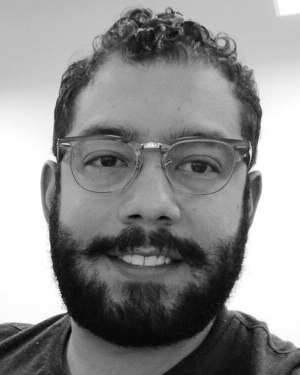
\includegraphics[width=1in,height=1.25in,clip,keepaspectratio]{../biography/yarib_300_375.jpg}}]{Yarib Nevarez} received the B.E. (Hons) degree in electronics from the Durango Institute of Technology, Durango, Mexico, in 2009, and the M.Sc. degree in Embedded Systems Design from the University of Applied Sciences Bremerhaven, Bremen, Germany, in 2017. He is currently pursuing a PhD degree with the Institute of Electrodynamics and Microelectronics, University of Bremen, Germany. His research interest is focused mainly on System-on-Chip architectures and hardware implementation for deep learning accelerators in Embedded Systems.
\\
During his professional experience, he served as a Senior Embedded Software Engineer at Texas Instruments, IBM, Continental Automotive, TOSHIBA, and Carbon Robotics. He has designed and developed software architectures for graphic calculators, automotive systems, robotic drivers, and more.
	
\end{IEEEbiography}

\begin{IEEEbiography}[{
\includegraphics[width=1in,height=1.25in,clip,keepaspectratio]{../biography/Beering_bw_klein.jpeg}}]{Andreas Beering} received his B.Sc. and M.Sc. degree in Electrical and Information Engineering  from the University of Bremen, Germany, in 2015 and 2017, respectively. He is currently working towards a Ph.D. degree at the Institute of Electrodynamics and Microelectronics at the University of Bremen, Germany. His research interests focus mainly on signal processing and classification of vibration signals. In addition to the analysis of passive acoustic emission for monitoring gearboxes and processes, the second focus lies on active ultrasonic investigations.
In this context, ultrasonic waveforms for monitoring overmoulding processes are being investigated.
\end{IEEEbiography}

\begin{IEEEbiography}[{
\includegraphics[width=1in,height=1.25in,clip,keepaspectratio]{../biography/person.png}}]{Amir Najafi}
\end{IEEEbiography}

\begin{IEEEbiography}[{
\includegraphics[width=1in,height=1.25in,clip,keepaspectratio]{../biography/person.png}}]{Ardalan Najafi}
\end{IEEEbiography}

\begin{IEEEbiography}[{
\includegraphics[width=1in,height=1.25in,clip,keepaspectratio]{../biography/wyu.jpg}}]{Wanli Yu}
	
	received the B. S. degree in information engineering and the M. S. degree in signal and information processing from the China University of Mining and Technology, Xuzhou, China, in 2009 and 2012, respectively and the PhD degree from the University of Bremen, Germany, in 2018.
	
	He is currently a Post-Doctoral Researcher with the Institute of Electrodynamics and Microelectronics, University of Bremen. His research interests include sensor networks, Internet of Things, network performance optimization, energy aware task allocation and scheduling, mobile edge/fog computing, convex optimization, machine learningand nature-inspired population-based optimization.
\end{IEEEbiography}

\begin{IEEEbiography}[{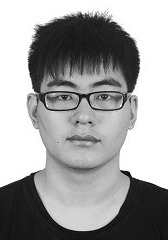
\includegraphics[width=1in,height=1.25in,clip,keepaspectratio]{../biography/YizhiChen.jpg}}]{Yizhi Chen} received the B.E. degree in Electronic and Information Engineering from Wuhan University, China, in 2017 and he received the M.S. degree in Communication and Information Technology from the University of Bremen, Germany, in 2021. Currently, he is working as a Ph.D. student at the Division of Electronics and Embedded Systems, Department of Electrical Engineering, School of Electrical Engineering and Computer Science, KTH Royal Institute of Technology, Sweden. His research interests include hardware accelerator for ML, fault-tolerant hardware for neural networks, Network-on-Chip, and approximate computing.
\end{IEEEbiography}

\begin{IEEEbiography}[{
\includegraphics[width=1in,height=1.25in,clip,keepaspectratio]{../biography/krieger.jpg}}]{Karl-Ludwig Krieger} received his Ph.D. degree in Electrical Engineering in 1999 from the University of Bremen, Germany. Dr. Krieger worked from 1998-2009 as a manager in the field of function and algorithm development for powertrain systems at Daimler AG in Stuttgart. Since 2009 he has been a full professor for the chair of Electronic Vehicle and Mobility Systems at the University of Bremen, Germany. The research focus of his chair is primarily on the analysis of vibration and ultrasound signals in different application fields, for example, passenger cars, heavy-duty trucks, mobile working machines or industrial machines. Further research priorities of the chair are near-infrared spectral sensors and capacitive sensor systems for different fields of application. These research topics are worked on in close cooperation with leading industrial partners and are mainly financed from third-party funds.
\end{IEEEbiography}

\begin{IEEEbiography}[{
\includegraphics[width=1in,height=1.25in,clip,keepaspectratio]{../biography/Alberto_Garcia-Ortiz.jpg}}]{Alberto Garcia-Ortiz}
    obtained the diploma degree in
    Telecommunication Systems from the Polytechnic University of
    Valencia (Spain) in 1998. After working for two years at Newlogic
    in Austria, he started the Ph.D. at the Institute of
    Microelectronic Systems, Darmstadt University of Technology,
    Germany. In 2003, he received from the Department of Electrical
    Engineering and Information Technology of the university the
    Ph.D. degree with "summa cum laude." From 2003 to 2005, he worked
    as a Senior Hardware Design Engineer at IBM Deutschland
    Development and Research in B{\"o}blingen.  After that he joined the
    start-up AnaFocus (Spain), where he was responsible for the design
    and integration of AnaFocus" next generation Vision
    Systems-on-Chip. He is currently full professor for the chair of
    integrated digital systems at the university of Bremen.
    Dr. Garcia-Ortiz received the "Outstanding dissertation award" in
    2004 from the European Design and Automation Association. In 2005,
    he received from IBM an innovation award for contributions to
    leakage estimation. Two patents are issued with that work. He
    serves as editor of JOLPE and is reviewer of several conferences,
    journals, and European projects. \\
    His interests include low-power
    design and estimation, communication- centric design, SoC
    integration, and variations-aware design. 
\end{IEEEbiography}


\EOD

\end{document}
